\bartchapterimage{heic0910i.jpg}
\chapter{Generating mock catalogues}
\label{cha:mock}
\bartthumb{heic0910i.png}

\minitoc%

\section{Introduction}

A mock catalogue is a useful tool to test galaxy group algorithms. These mocks
can reproduce many properties of galaxies, e.g.\ clustering, luminosity
function, etc, and add observational effects such as incompleteness and
measurement errors. There are different methods to obtain such a mock
catalogue. All of them involve cosmological simulations of dark matter halos.
According to the model of galaxy formation, we can use the halo occupation
distribution (HOD) to populate dark matter haloes with galaxies and putting
some luminosity functions (for example) as constraints. We can, alternatively,
follow galaxies in semi-analytical models (SAM) in cosmological simulations
outputs in order to have statistical properties of galaxies that agree with
observational results. With such realistic galaxies, we can use those
simulation boxes to place an observer into it, and create a mock survey. But to
have a realistic mock catalogue, it's necessary to take care of many things
which will be described in the next section.

\section{Populating dark matter halos}
\label{sec:populating_dark_matter_halos}

The first step in the construction of a galaxy mock catalogue is to populate
galaxies inside their dark matter halos, according to the model of the galaxy
formation and the constraints imposed by the observations. The real large scale
structure of the Universe is not directly observable and we must be confident
in the different cosmological simulation code outputs available to get the
distribution of dark matter halos. For example, there is the Millennium-II run
\citep{BoylanKolchin+09} of $2160^3$ dark matter particles, with a simulation
box size of 100 $h^{-1} \mathrm{Mpc}$ allowing a relatively high resolution for
the particles mass ($6.9\;10^6\;h^{-1} M_\odot$) and a precise determination of
the halo mass function and the history of each individual halo. Several
cosmological simulation codes exist to follow the dark matter particle
distribution along the evolution of the Universe \citep{Springel+01,
Teyssier+02, Springel+05}.

From the outputs of this cosmological simulations, informations on dark matter
halos are extracted using halo finder codes \citep{KK+09, Tweed+09,
Planelles+10}. Several methods exist to identify such structures: the
Friend-of-Friends approach \citep{Davis+85} that tends to link between them
different halos by bridges of linked dark matter particles, and doesn't
identify sub-halos; the spherical over-density measuring the density field and
searching around density peaks iteratively until the desired density threshold
is reached \citep{PS+74}; \textsc{Subfind} of~\cite{Springel+01} is similar to
FoF with peaks searched within the extracted FoF halos\ldots With all available
informations on halos, they can be populated by galaxies with prescriptions of
the galaxy formation model.

\subsection{Halo occupation distribution}
\label{sub:halo_occupation_distribution}

In the Halo Occupation Distribution method \citep{MS02,BW02,Zehavi+11}, the
galaxy richness in groups is deduced on a probability distribution function
depending on the halo mass, and their physical properties such as luminosity
from conditional luminosity functions depending on the dynamical mass too
\citep{YMvdB03}. A relation between the galaxy and matter distribution is
imposed by three constraints: the probability distribution $P \left(N|M\right)$
that a halo of mass $M$ contains $N$ galaxies, the spatial relation between the
galaxy and dark matter, and the same for the velocity distribution. The galaxy
distribution is assumed to be spherically symmetric, and follows that of the
dark matter particles in the halos of $\Lambda$CDM cosmological simulations
(e.g., NFW), the velocities are drawn from Maxwellian distributions (see
\citealp{Beraldo+14} for the limitations of this assumption), with radial and
tangential velocity dispersions derived from the Jeans equation of local
dynamical equilibrium, assuming some form for the radial variation of the
velocity anisotropy.

\subsection{Semi-analytical models}
\label{sub:semi_analytical_models}

In  Semi-Analytical Models (SAMs, e.g., \citealp{RQPR97,KCDW99}), galaxy
properties (in particular stellar mass and $r$-band luminosity) are painted on
the halos and subhalos of cosmological $N$ body simulations across cosmic time,
following well-defined physical recipes for star formation and galaxy feedback.
This procedure produces galaxies that follow relatively well the observed
luminosity, stellar mass functions and scaling relations.

We have chosen this second approach, because the recent SAM by~\cite{Guo+11},
run on the Millennium-II simulation \citep{BoylanKolchin+09} fits well the
$z$=0 observations (as shown by \citeauthor{Guo+11}). The Millennium-II
simulation  involved $2160^3$ particles in a box of comoving size 137 Mpc,
running with cosmological parameters $\Omega_{\rm m}=0.25$,
$\Omega_\Lambda=0.75$, $h=0.73$, and $\sigma_8=0.9$. The particle mass was thus
$9.5\times 10^6 M_\odot$.

We extracted the SAM output of~\cite{Guo+11} from the Guo2010a database on the
German Astrophysical Virtual Observatory
website.~\footnote{http://gavo.mpa-garching.mpg.de/Millennium/Help,
see~\cite{Lemson06}} The real-space groups were extracted by
\citeauthor{Guo+11} using the FoF technique applied to the particle data, with
over $10^5$ particles for groups of mass $>10^{12} \rm M_\odot$. The database
includes the mass within the sphere of radius $r_{200}$, where the mean mass
density is $\Delta=200$ times the critical density of the Universe, centered on
the particle in Millennium-II simulation, within the largest sub-halo, with the
most negative gravitational potential \citep{BoylanKolchin+09}. We slightly
modified the membership of the true groups by considering only the galaxies
within $r_{200}$.\footnote{We kept the galaxies outside the sphere of radius
$r_{200}$ as possible interlopers.}

\section{Mock structure}

In all this section, we will assume that we have already in our possession a
dark matter simulation box which has been populated with galaxies with one of
the methods described below (SAM, HOD\ldots). At this step, physical properties
of those galaxies aren't interesting.

\subsection{Placing boxes}

The first step to make a mock catalogue is to get galaxies positions like in a
survey, to get an $(\alpha,\delta)$ frame to simulate the sky coverage of
survey.

The mock catalogue must have the same volume as the galaxy survey we want to
mimic. For example for the SDSS survey, we can measure redshift to a value of
0.3 and more. But the problem is that the majority of the simulation boxes have
a size of around $L_{\mathrm{box}}=100-300\; h^{-1}$ Mpc, letting us with a
maximal redshift in our mock survey of around ${H_0}{L_{\mathrm{box}}}/c\approx
0.025$ in the case of a box of $100\; h^{-1}$ Mpc in size. Bigger simulations
exist, and allow us to access higher redshifts, but this increasing size
reduces the resolution of the simulation in particle mass and therefore we
cannot have low mass halos in the simulations.

The solution is to take a ``little'' simulation box and to replicate it and to
make some ``Tetris'' cube until we reach the maximal redshift we want. An
example of the resulting ``mock cube'' is shown on \bartreffigure{cubemock}.
%
\begin{figure}[htb]
    \centering
    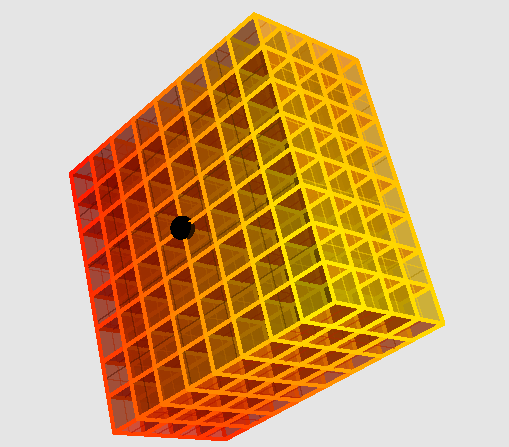
\includegraphics[width=0.4\linewidth]{figures/mock/mock}
    \caption{The structure of the mock catalog once we have replicated the
        simulation box chosen to populate dark matter halos. Each cube
        represents a simulation box whose galaxies were randomly rotated and
        translated in positions. Placing an observer at a given position (the
    black dot), we can access different geometries for the survey and go to
higher redshift ranges than those possible with an unique simulation
box.\label{fig:cubemock}}%
\end{figure}

Now, if we take an observer at some position into this big box, we can have
different sky coverage for the observer. The simplest is to place the observer
at a corner, which gives a solid angle of $\pi/2$ steradians. At the centre,
we have a full sky coverage but we reduce the redshift extension by two. For
the SDSS, as in \bartreffigure{cubemock}, the area of the survey is large (see
\bartrefappendix{sdss}) and we need to cover half of the sky to get the same
volume.

If we want to care about redshift evolution of galaxies for the observer, we
need to use other snapshots at different redshifts, simply joining cubes in
comoving coordinates. Indeed, the cosmological redshift of the galaxy is
deduced from the relation between the redshift and its comoving distance,
equals to the comoving transverse distance (or proper motion distance) in the
case of a flat Universe $\Omega_k=0$ \citep{Hogg+99}. Moreover, the comoving
separation $R_c$ between two points with angular separation $\theta$ on the
sky, at comoving distance $D_c$ from the observer, are simply related by a
geometrical relation $R_c=\theta D_c$. This separation $\theta$ deduced from
comoving coordinates should be the same as those of the observer working with
physical coordinates. The observer wants to know the physical separation $R_p$
between the two galaxies, so $R_p=\theta d_\mathrm{ang}$ giving $R_p
\left(1+z\right)= R_p/a\left(z\right)=R_c=\theta D_c$ (where $a \left(z\right)$
is the scale factor with $a \left(0\right)=1$).

Placing boxes as described previously creates a perspective effect from the
point of view of an observer \citep{Blaizot+05}, and the consequences aren't
predictable in a statistical sense. To avoid this, we apply some coordinate
transformations on galaxies in the initial cube like inversions, rotations and
periodic translations. Rotations are multiples of $\pi/2$ around the three
principal coordinates axes, because if other rotations are allowed, this create
over-densities in some regions of the final mock which aren't physical.
Translations are performed on the three principal axes and when galaxies are
out of the initial cube, periodic conditions are applied. All of those
transformations are randomly generated for each cube in the final mock
catalogue.

\subsection{Physics}

\subsubsection{Celestial coordinates}

The first step to simulate this is to transform Cartesian coordinates ($X, Y,
Z$) in the 3D space to celestial coordinates ($(\alpha,\delta)$ frame). In our
case, the origin of coordinates is the observer. Getting these coordinates is
the same as computing spherical coordinates.
%
\begin{equation}
    \alpha=\mbox{arctan2} \left(Y, X\right) \mod 2\pi
    \nonumber%
\end{equation}
%
\begin{equation}
    \delta=\mbox{sgn} \left(Z\right)
    \arccos\left(\frac{\sqrt{X^2+Y^2}}{\sqrt{X^2+Y^2+Z^2}}\right)
\end{equation}
%
where $\mbox{sgn}$ is the sign function\footnote{For the sign function:
    \begin{equation}
        \mbox{sgn}(x)= \begin{cases}
            1 &\mbox{if} \; x > 1 \\
            -1 &\mbox{if} \; x < 1 \\
            0 &\mbox{else}
        \end{cases}
    \end{equation}
%
and the $\mbox{arctan2}$ function is:
%
    \begin{equation}
        \mbox{arctan2} \left(y, x\right) = \begin{cases}
            \phi \times\mbox{sgn}(y) & x > 0 \\
            \cfrac{\pi}{2} \times\mbox{sgn}(y) & x = 0 \\
            \left(\pi - \phi\right) \times\mbox{sgn}(y) & x < 0
        \end{cases}
    \end{equation}
%
with $\tan\phi = \left|\cfrac{y}{x}\right|$ particular cases:
%
    \begin{equation}
        \mbox{arctan2} \left(0, x\right) = \begin{cases}
            0 & x > 0 \\
            \mbox{not defined} & x = 0 \\
            \pi & x < 0
        \end{cases}
    \end{equation}
}

\subsubsection{Redshifts}

If we keep the distance as calculated previously, the observer can still have
precise determination of the distance of a galaxy. In reality, we observe it in
redshift space so the redshift as distance indicator is biased by peculiar
velocities. Our initial galaxy catalog allows us to get the velocity of a
galaxy, so we compute the line of sight (los) velocity of this galaxy
relatively to the observer.
%
\begin{equation}
v_\mathrm{los}=\cfrac{\textbf{OG}.\textbf{v}_\mathrm{pec}}
    {\left|\left|\textbf{OG}\right|\right|}
\end{equation}
%
where $O$ is the observer and $G$ the galaxy, $\textbf{v}_{\mathrm{pec}}$ its
peculiar velocity. This velocity has a sign. The redshift is just the
expression of a shift in wavelength. The observed wavelength $\lambda$ is
linked to the original (emitted) wavelength $\lambda_0$ by:
%
\begin{equation}
    \lambda=(1+z)\lambda_0
\end{equation}
%
The shift caused by Universe expansion is
$\lambda_{\cos}=(1+z_{\cos})\lambda_0$ where the subscript $\cos$ refer to the
cosmological expansion. The shift caused by the peculiar velocity is
$\lambda=(1+z_{\mathrm{pec}})\lambda_{\cos}$. So the observed wavelength is
$\lambda=(1+z_{\mathrm{pec}})(1+z_{\cos})\lambda_0$. The resulting observed
redshift is:
%
\begin{equation}
    (1+z)=(1+z_{\mathrm{pec}})(1+z_{\cos})
\end{equation}
%
The peculiar redshift is the relativistic Doppler effect:
%
\begin{equation}
    (1+z_{\mathrm{pec}})=\sqrt{\cfrac{1+\beta}{1-\beta}}
\end{equation}
%
with $\beta={v_{\mathrm{los}}}/{c}$. The cosmological redshift is approximated
by $z_{\cos}={H_0}{D}/c$ where $D$ is the physical distance of the galaxy to
the observer and $H_0$ the Hubble constant, in the case of a simple computation
of the redshift. We can also make a more precise computation by searching the
solution of $D=d_\mathrm{pm} \left(z_{\cos}\right)$ with $d_\mathrm{pm}
\left(z\right)$ the proper motion distance at the redshift $z$.

Applying this method to mock catalogue, we can have galaxies whose ``distance''
is biased by peculiar velocities in redshift space. With such a treatment, the
velocity dispersion of galaxies in groups leads to the apparition of ``fingers
of God'', an elongation of galaxy groups along the line-of-sight, as in
redshift space observations.

We don't have to add the wavelength shift due to the translation of the
observer relatively to the Cosmological Microwave Background (CMB). Velocities
in the simulation are relative to an ``absolute'' frame, but our Galaxy has a
movement in relation to the CMB creating an additional shift in wavelength
depending on the observed region of the celestial sphere, and we should include
it in our mock catalogue. But frequently, redshifts accessible in galaxy
surveys are already corrected for the CMB relative motion, or can be easily
pre-corrected to avoid this component. In consequence, we don't integrate it in
our mock catalogue.

\subsubsection{Survey mask}

With our frame in redshift space relative to the observer, we can apply
different masks on angular coordinates according to the survey we want to
mimic. An example of such a mask is in \bartrefchapter{sdss}, where we describe
how to decide if a galaxy is inside the mask or not, in the case of the SDSS\@.

\subsubsection{K-corrections}

In reality, an observer studies galaxies in a given bandwidth in wavelength and
can't use the bolometric flux of the object. With the expanding Universe, all
the spectral energy distribution (SED) of galaxy is shifted. All wavelengths
are shifted by the same value for a given redshift. So, knowing the luminosity
$L$ of a galaxy in a given band in reality (using the true SED), computing its
apparent magnitude for an observer aren't as easy as correcting for the
distance modulus. The observer in a given band sees a different part of the
rest frame SED\@. The flux observed in the same band as the rest frame flux is
maybe higher or lower. A correction for this effect is needed in the real
galaxy survey to estimate the distance of an object and must be taken into
account in our mock catalogue.

As explained before, this correction depends on the SED of galaxies and the
band used in the survey. The common way of correcting, it when we have a
multi-band photometry, is to fit the observed SED in those bands with
theoretical templates of SEDs. Such templates can be obtained with existing
programs as PEGASE \citep{LeBorgne+04}, giving us galaxy SEDs. But those
programs are a little time consuming, a problem for mock when we want to run
several of them. A quick alternative solution is provided by
\citet{Chilingarian+10}, where the K-correction is fitted on templates for SEDs
as given by PEGASE in terms of a 2D polynomial of the redshift of the galaxy
and its colour. The corresponding K-correction is precise for redshifts until
0.3 in different survey bands (including $ugriz$ for the SDSS). This work
reduces the computation of K-corrections to the use of simple polynomial
relations and make our task easier.

By definition, the K-correction $K$ for a galaxy of apparent magnitude $m_X$
in a given band $X$ and absolute magnitude $M_X$ in the same band is:
%
\begin{equation}
    m_X=M_X + 5\log_{10}\left(d_\mathrm{lum}\left[\mathrm{pc}\right]\right) - 5 + K
\end{equation}
%
In our case, the K-correction depends on the redshift of the galaxy and its
colour in apparent magnitude given two bands. So we can rewrite:
%
\begin{equation}
    \label{eq:appmag}
    m_X=M_X +
        5\log_{10}\left(d_\mathrm{lum}\left[\mathrm{pc}\right]\right) - 5 +
        K\left(z, m_X - m_{X'}\right)
\end{equation}
%
where:
%
\begin{equation}
    K\left(z,m_X-m_{X'}\right)=\sum_{i=0}^{N_i}\sum_{j=0}^{N_j} a_{ij} z^i
    {\left(m_X-m_{X'}\right)}^j
\end{equation}
%
and $a_{ij}$ is a $N_i\times N_j$ matrix containing the coefficients of the
two dimensional polynomial. These coefficients depend on the bands of the
survey used for the colour computation.

The observer in the mock can just, in theory, access to apparent magnitude of
the survey. But we don't know in advance these magnitudes, and as we can see in
the expression of \bartrefequation{appmag}, we need apparent magnitudes to
compute apparent magnitudes. If we use the other bands of the survey, with
$a_{ij}$ coefficients, we can always write a set of equations for a galaxy
which involves all apparent magnitudes of the survey. So we can write a set of
non linear equations with polynomial of order $N_j$ (redshift of the galaxy is
supposed to be known). Numerically it's easy to solve this set of equations,
and relatively fast with equations solvers or by iterations. In practice, the
first is faster than the second method, even if both methods give similar
results in apparent magnitudes.

\subsubsection{Flux limit}

We will see in \bartrefchapter{sdss} that spectroscoped galaxies are defined
for galaxies whose apparent magnitude is less than 17.77 in the $r$ band. So,
in all the redshift sub-samples, we will miss galaxies that are not
sufficiently bright. To take into account this effect, we remove galaxies not
reaching the limit apparent magnitude of the survey. An additional selection on
surface brightness is also done in the SDSS, but estimating this is difficult
from virtual galaxy catalogs and the number of ``lost'' galaxies is
sufficiently low to ignore this step in the construction of the mock catalog.

\subsubsection{Spectroscopic and photometric redshifts}

Sometimes, we don't have access to spectroscopic redshifts, but only to less
precise photometric redshifts. In the SDSS, for example, this is due to tiling
process. Fibers analysing the spectrum of galaxies cannot be closer from each
other than $55''$, so if for a target galaxy (selected to obtain a spectrum)
there is an other galaxy closer than those 55'', the tile containing all fibers
doesn't have the possibility to measure the redshift of this galaxy. A very
good algorithm to place tiles in order to limit the number of missed galaxies
(i.e.\ the number of fiber collision) has been applied to the galaxy sample of
the SDSS \citep{Blanton+03}. But there is still some galaxies without
spectroscoped redshifts, especially in dense regions such as the cases of
groups and clusters. If we remove those galaxies from our sample, there
will be a spectroscopic incompleteness with unknown effects on our results.

Unfortunately, there is no simple way to simulate this in the mock catalogue
and we choose to ignore it. Just a small fraction of galaxies are not
spectroscoped and this must not affect our results, when we will apply galaxy
group algorithms on a real galaxy survey.

\subsubsection{Observational errors}

The way we organized the construction of the mock catalogue is useful for the
introduction of observational errors. For example, we treat the case where we
want to add errors on the absolute magnitude of galaxies in the final mock
catalog. If we have a model for introducing such errors according to some
physical galaxy properties in the virtual galaxy catalogue, we can just add
them inside this virtual catalogue and magnitude errors will be reported on the
mock galaxy catalogue. If errors depend on properties computed in the mock
catalogue, we can simply add magnitude errors while constructing the mock
catalogue. Any kind of errors can be added such as redshift measurement errors,
astrometry, photometry, etc.

\subsection{Galaxy samples}
\label{sub:galaxy_samples}

\subsubsection{Definition}
\label{ssub:galaxy_sample_definition}

All previous steps lead to a final galaxy mock catalogue, with or without
observational errors, flux limited at a given apparent magnitude. But working
with flux limited samples requires correcting for missing galaxies when
extracting galaxy groups. The only way to avoid errors introduced by the
different choices of the model is to work with a doubly complete sample of
galaxies: limited in luminosity and in volume, thus avoiding completeness
issues.
%
\begin{figure}[htb]
    \centering
    \begin{minipage}{0.49\linewidth}
        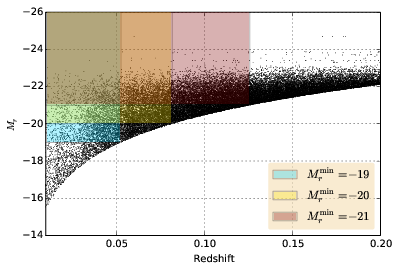
\includegraphics[width=\linewidth]{figures/mock/subsamples.png}
        \captionof{figure}{An illustration of the doubly complete galaxy
            samples used. Black dots represent galaxies in the mock catalogue.
            Colored rectangles show samples for a threshold absolute magnitude
            in the $r$ band $M_r$ of -19, -20, -21. Their sizes reflects the
        corresponding limits of the minimal luminosity. As we can see, in these
    regions, there is no need to correct for missing galaxies. All galaxies
above the given threshold magnitude are visible.\label{fig:subsamples}}
    \end{minipage}
    \begin{minipage}{0.49\linewidth}
        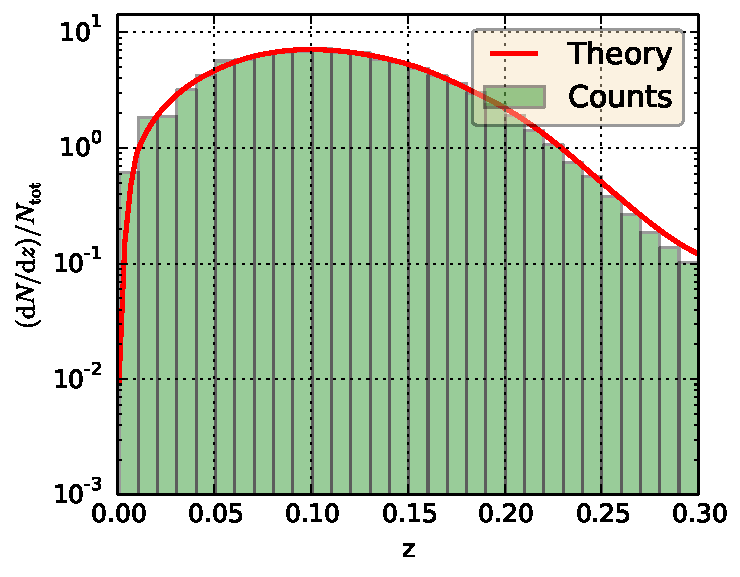
\includegraphics[width=\linewidth]{figures/mock/counts.pdf}
        \captionof{figure}{Comparison of counts in redshift of galaxies in the
            mock catalog with the theoretical expectation deduced from the
            number density of galaxies. In \emph{red} the theory and in
            \emph{green} counts directly done on the mock catalog. The small
            discrepancies observed at high redshift are caused by an
            imprecision in the computation of the integrated luminosity
            function, since we use an interpolation of the luminosity function,
        and only few bright galaxies at high redshift are visible making the
    integration difficult.\label{fig:counts}}
    \end{minipage}
\end{figure}

We choose a minimal galaxy luminosity for our sample and the maximal redshift
is computed with the maximal distance at which we can observe a galaxy with
this minimal luminosity. We note that if K-correction is considered, this limit
depends on the considered galaxy. A clean definition of the sample in this
situation should be done by restricting a little more the redshift extent to
not lose fainter galaxies. But the galaxy loss is low and we didn't consider
such a case. In \bartreftable{samples}, we show the six galaxy samples that we
constructed from our flux limited galaxy mock catalogue, with statistics on
each of them.
%
\begin{table}[htb]
    \caption{Doubly complete mock galaxy subsamples\label{tab:samples}}
    \begin{center}
    \setlength{\tabcolsep}{3pt}
    \begin{tabular}{lccccccc}
    \toprule
    \toprule
    ID & $M_r^{\max}$ & $L_r^{\min}/L*$ & $z_{ \max }$ & Number & $n$
    & $n^{-1/3}$ & Fraction\\
              &            &     &                 &        & ($\rm  Mpc^{-3}$)
    & (Mpc) & split\\
    \toprule
    1 & --18.5 & 0.09 & 0.042 & \ \,47158 & 0.0125 & 4.32 & 5.3\%\\
    2 & --19.0 & 0.14 & 0.053 & \ \,72510 & 0.0099 & 4.66 & 6.1\%\\
    3 & --19.5 & 0.22 & 0.066 & 112629    & 0.0078 & 5.05 & 6.6\%\\
    4 & --20.0 & 0.36 & 0.082 & 166899    & 0.0058 & 5.56 & 7.4\%\\
    5 & --20.5 & 0.56 & 0.102 & 213546    & 0.0040 & 6.29 & 8.6\%\\
    6 & --21.0 & 0.90 & 0.126 & 245821    & 0.0025 & 7.40 & 9.9\%\\
    \bottomrule
    \end{tabular}
    \end{center}
    \parbox{\hsize}{\footnotesize Notes: Columns are: sample, maximum $r$-band absolute
    magnitude, minimum luminosity in units of $L*$ (adopting $M*=-20.44 +
    5\,\log h$ in the SDSS $r$ band from \citealp{Blanton+03}), maximum
    redshift, sample size, mean density $n$, proxy for the mean separation to
    the closest neighbor, $n^{-1/3}$, and the percentage of true groups that
    are flagged because they are split during the simulation box
    transformations. The minimum redshift of each subsample is $z=0.01$.
}
\end{table}

\subsubsection{Limitations}
\label{ssub:galaxy_samples_limitations}

The mock catalogue is constructed from the adjoining of multiple simulation
boxes, each of them having periodic boundaries. A consequence is that some
galaxy groups are split by a simulation box size, and from the point of view of
the observer, members are at two different locations on the celestial sphere.
Inclusion of such groups in statistics leads to biased results of the
performance of grouping algorithms, and a flag is used to distinguish and
remove such groups.

Moreover, the limited volume extension of the survey truncates some groups. In
redshift space, these limits are of two kinds: the angular mask cutting groups
all along the line-of-sight (i.e.\ survey edges and possibly holes), and the
redshift cut with a more important effect due to the elongation in redshift
coordinates by the intrinsic velocity dispersion of the system. Since all the
information on the group is not accessible by the observer, estimation of group
properties is less precise. To avoid the degradation of the performances of
grouping algorithms, we flag selected groups (after the application of a
grouping algorithm) if they are close to edges of the angular mask or edges in
depth (see \bartrefchapter{friends_of_friends_algorithm} for a detailed
definition) and remove them from the statistics in tests.

\section{Validity}
\label{sec:validity}

Finally, we test the construction of our mock catalogue with a simple
comparison with the expectation from the theoretical redshift counts. Indeed,
the redshift count is:
%
\begin{equation}
    \label{eq:counts}
    \cfrac{\dd N}{\dd z} = \cfrac{\dd N}{\dd V}\times\frac{\dd V}{\dd z}
\end{equation}
%
where $V$ is the comoving volume.
The first term of the \emph{rhs} of \bartrefequation{counts} is just the integrated luminosity function
$\Phi$:
%
\begin{equation}
    \cfrac{\dd N}{\dd V} = \int_{L_{\lim} \left(z\right)}^\infty
    \cfrac{\dd^2 N}{\dd V \dd L}\dd L = \int_{L_{\lim} \left(z\right)}^\infty \Phi \left(L\right)\dd L
\end{equation}
%
The luminosity function is directly deduced from the virtual galaxy catalog of
\citet{Guo+11}.

The second term of the \emph{rhs} of \bartrefequation{counts} is the variation
of the comoving volume with redshift (see \citet{Hogg+99}):
%
\begin{equation}
    \cfrac{\dd V}{\dd z} = D_{\rm H} \cfrac{{d_{\rm pm} \left(z\right)}^2}
    {E\left(z\right)} \dd \Omega
\end{equation}
%
where $\dd\Omega$ is the elemental solid angle, $d_{\rm pm}$ the proper motion
distance (or comoving distance, see \bartrefappendix{formulas}), $D_H$ the
Hubble distance $c/H_0$ and $E\left(z\right)$ the evolution of the Hubble
constant with the redshift. The result of the theoretical prediction and the
comparison with the obtained mock catalog is shown in \bartreffigure{counts}.

% vim: set tw=79 :
